% !TEX root = task-1-1-1.tex
% Editable task bank. Append new BankTask blocks at the end of the document.
\documentclass[12pt,a4paper]{article}
\usepackage{physics-textbook}
\usepackage{graphicx,needspace}
\usetikzlibrary{decorations.pathmorphing}
\newif\ifShowSolutions
\ifdefined\TutorEdition
  \ShowSolutionstrue
\else
  \ShowSolutionsfalse % Change to \ShowSolutionstrue to display solutions.
\fi
\newcounter{banktask}
\newsavebox{\BankTaskBox}
\newcommand{\BankTaskContent}[3]{%
  \noindent\textbf{\thebanktask.}\quad #2\par
  \ifShowSolutions
    \Needspace{50mm}% Keep the solution heading with its opening text or diagram.
    #3\par
    \ifdefined\TutorEdition
      \ifcsname TutorSource#1\endcsname
        \nopagebreak\smallskip{\small\csname TutorSource#1\endcsname\par}%
      \fi
    \fi
  \fi
}
\newcommand{\BankTask}[3]{%
  \refstepcounter{banktask}\par\medskip
  \sbox{\BankTaskBox}{\begin{minipage}{\linewidth}%
    \BankTaskContent{#1}{#2}{#3}\end{minipage}}%
  \ifdim\dimexpr\ht\BankTaskBox+\dp\BankTaskBox\relax>\dimexpr\textheight-20mm\relax
    \Needspace{35mm}\BankTaskContent{#1}{#2}{#3}%
  \else
    \Needspace{\dimexpr\ht\BankTaskBox+\dp\BankTaskBox\relax}%
    \noindent\usebox{\BankTaskBox}\par
  \fi
  \medskip
}
\begin{document}
\BookSubsection{1.1.1}{Относительность движения}


% Source sdamgia-125: https://phys-ege.sdamgia.ru/problem?id=125
\BankTask{sdamgia-125}{
Вертолет поднимается вертикально вверх. Какова траектория движения точки на конце лопасти винта вертолета в системе отсчета, связанной с винтом?

$1$) точка

$2$) прямая

$3$) окружность

$4$) винтовая линия
}{
\smallskip\noindent\textbf{Решение}\par
В системе отсчета, связанной с винтом, точка на конце лопасти не двигается. Следовательно, ее траектория в данной системе отсчета представляет собой точку.

Ответ: $1$.
}

% Source sdamgia-3357: https://phys-ege.sdamgia.ru/problem?id=3357
\BankTask{sdamgia-3357}{
Вертолет равномерно поднимается вертикально вверх. Какова траектория крайней точки лопасти вертолета в системе отсчета, связанной с корпусом вертолета?

$1$) прямая линия

$2$) винтовая линия

$3$) окружность

$4$) эллипс
}{
\smallskip\noindent\textbf{Решение}\par
Крайняя точка лопасти вертолета двигается по окружности вокруг оси вращения винта. Поскольку ось вращения жестко связана с корпусом вертолета, такую же траекторию описывает эта точка и относительно любой точки корпуса.

Ответ: $3$.
}

% Source sdamgia-5952: https://phys-ege.sdamgia.ru/problem?id=5952
\BankTask{sdamgia-5952}{
Два камня одновременно бросили из одной точки: первый — вертикально вверх, второй — под углом $45^\circ$ к горизонту. Сопротивление воздуха пренебрежимо мало. Как движется первый камень в системе отсчета, связанной со вторым камнем?

$1$) покоится

$2$) движется по параболе

$3$) движется равномерно и прямолинейно

$4$) движется по дуге окружности
}{
\smallskip\noindent\textbf{Решение}\par
Перейдем в систему отсчета, связанную со вторым камнем. Первый камень движется относительно Земли с ускорением, одинаковым по величине и направлению ускорению второго камня, следовательно, ускорения в системе отсчета, связанной со вторым камнем, он не имеет, значит, его движение равномерно и прямолинейно.

Правильный ответ указан под номером $3$.
}

% Source sdamgia-6637: https://phys-ege.sdamgia.ru/problem?id=6637
\BankTask{sdamgia-6637}{
Маша взяла в руку монету и, стоя в комнате своей квартиры, выпустила ее из пальцев без начальной скорости. Монета полетела вдоль вертикали и упала на пол комнаты. Затем Маша вышла из дома, села в подъехавший автобус и, дождавшись, пока он начнет двигаться равномерно и прямолинейно по горизонтальной дороге, повторила опыт с бросанием монеты. Оказалось, что монета в равномерно движущемся автобусе падает точно так же, как и в квартире. Иллюстрацией какого закона или принципа может служить этот опыт?

$1$) первого закона Ньютона

$2$) второго закона Ньютона

$3$) третьего закона Ньютона

$4$) принципа относительности Галилея
}{
\smallskip\noindent\textbf{Решение}\par
Этот опыт является иллюстрацией принципа относительности Галилея, который гласит, что в любых инерциальных системах отсчета все механически процессы проходят одинаково. 

Ответ: $4$.
}

% Source sdamgia-6038: https://phys-ege.sdamgia.ru/problem?id=6038
\BankTask{sdamgia-6038}{
Мотоцикл едет по прямой дороге с постоянной скоростью $50\,\text{км/ч}$. По той же дороге навстречу ему едет автомобиль с постоянной скоростью $70\,\text{км/ч}$. Чему равен модуль скорости движения мотоцикла относительно автомобиля? (Ответ дайте в километрах в час.)
}{
\smallskip\noindent\textbf{Решение}\par
Перейдем в систему отсчета, связанную с автомобилем. Модуль скорости движения мотоцикла в данной системе отсчета будет равен $50 + 70 = 120\,\text{км/ч}$.

Ответ: $120$.
}

% Source sdamgia-3548: https://phys-ege.sdamgia.ru/problem?id=3548
\BankTask{sdamgia-3548}{
Пешеход идет по прямолинейному участку дороги со скоростью $4\,\text{км/ч}$. Навстречу ему движется автобус со скоростью $40\,\text{км/ч}$. С какой скоростью (в км/ч) должен двигаться навстречу пешеходу велосипедист, чтобы модуль его скорости относительно пешехода и автобуса был одинаков?
}{
\smallskip\noindent\textbf{Решение}\par
Обозначим искомую скорость велосипедиста через $v .$ Тогда, как видно из рисунка, велосипедист приближается к пешеходу со скоростью $v + 4,$ а к автобусу — со скоростью $40 - v .$

\begin{center}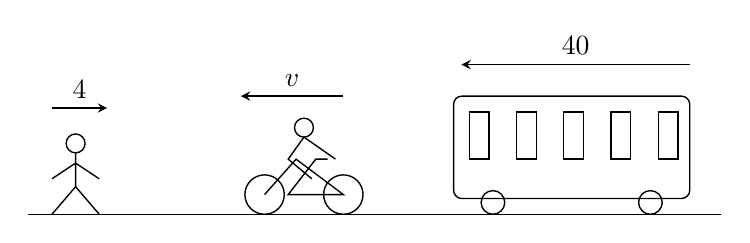
\begin{tikzpicture}[>=stealth,line width=.5pt]

\draw(-.4,0)--(8.4,0);
\draw(.2,.9)circle(.12);\draw(.2,.78)--(.2,.35)--(-.1,0) (.2,.35)--(.5,0) (.2,.65)--(-.1,.45) (.2,.65)--(.5,.45);
\draw[->](-.1,1.35)--(.6,1.35)node[midway,above]{$4$};
\draw(2.6,.25)circle(.25) (3.6,.25)circle(.25);\draw(2.6,.25)--(3,.7)--(3.6,.25)--(2.9,.25)--(3.25,.7)--(3.4,.7);\draw(3.1,1.1)circle(.12);\draw(3.1,.98)--(2.9,.7)--(3.2,.45) (3.1,.98)--(3.5,.7);
\draw[->](3.6,1.5)--(2.3,1.5)node[midway,above]{$v$};
\draw[rounded corners=3pt](5,.2)rectangle(8,1.5);\foreach\x in{5.2,5.8,6.4,7,7.6}\draw(\x,.7)rectangle(\x+.25,1.3);\draw(5.5,.15)circle(.15) (7.5,.15)circle(.15);
\draw[->](8,1.9)--(5.1,1.9)node[midway,above]{$40$};
\end{tikzpicture}\end{center}

Приравняв эти две скорости, находим требуемую скорость велосипедиста: $v + 4=40 - v \Longleftrightarrow  v =18\,\text{км/ч}.$

Ответ: $18$.
}

% Source sdamgia-3549: https://phys-ege.sdamgia.ru/problem?id=3549
\BankTask{sdamgia-3549}{
Пароход движется по реке против течения со скоростью $5\,\text{м/с}$ относительно берега. Определите скорость течения реки, если скорость парохода относительно берега при движении в обратном направлении равна $8\,\text{м/с}$. (Ответ дайте в метрах в секунду.)
}{
\smallskip\noindent\textbf{Решение}\par
Обозначим искомую скорость течения реки через $u$, а скорость парохода в стоячей воде — через $v .$ Тогда можно составить следующие уравнения. Скорость парохода вниз по течению равна $v + u=8\,\text{м/с}.$ Скорость парохода вверх по течению: $v - u=5\,\text{м/с}.$ Решая систему из двух этих уравнений, для скорости течения воды имеем $u=1{,}5\,\text{м/с}.$

Ответ: $1{,}5$.
}

% Source sdamgia-11807: https://phys-ege.sdamgia.ru/problem?id=11807
\BankTask{sdamgia-11807}{
Расстояние между пунктами А и В равно $30\,\text{км}$. Из пункта А в направлении пункта В выезжает мотоциклист со скоростью $50\,\text{км/ч}$. Одновременно из пункта В в том же направлении, что и мотоциклист, выезжает трактор со скоростью $20\,\text{км/ч}$. На каком расстоянии от пункта А мотоциклист догонит трактор? Ответ приведите в километрах.
}{
\smallskip\noindent\textbf{Решение}\par
Для того чтобы догнать трактор, мотоциклисту нужно сократить расстояние в $30\,\text{км}$. Относительная скорость мотоциклиста относительно трактора равна $50\,\text{км/ч} - 20\,\text{км/ч} = 30\,\text{км/ч}$. Следовательно, мотоциклист догонит трактор за $\frac{30\,\text{км}}{30\,\text{км/ч}} = 1\,\text{ч}.$ За это время мотоциклист проедет $50\,\text{км}$.

Ответ: $50$.
}

% Source sdamgia-2915: https://phys-ege.sdamgia.ru/problem?id=2915
\BankTask{sdamgia-2915}{
В безветренную погоду самолет затрачивает на перелет между городами $6\,\text{часов}$. Если во время полета дует постоянный боковой ветер перпендикулярно линии полета, то самолет затрачивает на перелет на $9$ минут больше. Найдите скорость ветра, если скорость самолета относительно воздуха постоянна и равна $328\,\text{км/ч}.$
}{
\smallskip\noindent\textbf{Решение}\par
Путь, пройденный самолетом в первом случае: $s=v_{\text{СВ}}t_1,$ где $v_{\text{СВ}}$ — скорость самолета относительно воздуха. 

\begin{center}\begin{tikzpicture}[>=stealth,line width=.5pt]

\node at(-.3,.15){I};\draw[dashed](0,0)--(3.5,0);\draw[->](.8,0)--(2.3,0)node[midway,above]{$\vec v_{\text{СВ}}$};
\begin{scope}[xshift=4.6cm]\node at(-.3,.15){II};\draw[dashed](0,0)--(3.5,0);\draw[->](.2,0)--(2.8,0)node[midway,below]{$\vec v_{\text{С}}$};\draw[->](.2,0)--(.2,1)node[left]{$\vec v_{\text{В}}$};\draw[->](.2,1)--(2.8,0)node[midway,above]{$\vec v_{\text{СВ}}$};\end{scope}
\end{tikzpicture}\end{center}

Закон сложения скоростей в векторном виде для перелета во время ветра: $\vec v_{\text{С}}=\vec v_{\text{СВ}}+\vec v_{\text{В}},$ где $\vec v_{\text{В}}$ — скорость ветра. Выражение для модуля скорости самолета относительно Земли во втором случае имеет вид: 

\[v_{\text{С}}=\sqrt{v_{\text{СВ}}^2-v_{\text{В}}^2}.\]

Тогда путь, пройденный самолетом во втором случае:

\[s=v_{\text{С}}t_2=\sqrt{v_{\text{СВ}}^2-v_{\text{В}}^2}\,t_2.\]

Следовательно: 

$v_{\text{СВ}}t_1=\sqrt{v_{\text{СВ}}^2-v_{\text{В}}^2}\,t_2.$ Отсюда: 

\[v_{\text{В}}=\frac{v_{\text{СВ}}\sqrt{t_2^2-t_1^2}}{t_2}.\]

Ответ: $v _B=72\,\text{км/ч}=20\,\text{м/с}.$
}

% Source sdamgia-9752: https://phys-ege.sdamgia.ru/problem?id=9752
\BankTask{sdamgia-9752}{
Скорость течения широкой реки $3{,}6\,\text{км/ч}$. Под каким углом к направлению течения реки лодочник должен направлять лодку, скорость которой относительно воды равна $2\,\text{м/с}$, чтобы за $15$ минут ее снесло по направлению течения на $1{,}8\,\text{км}$?
}{
\smallskip\noindent\textbf{Решение}\par
При движении под углом $\alpha $ к течению реки, лодка будет двигаться по реке со скоростью 

\[V=V_{\text{теч}}+V_{\text{л}}\cos\alpha=3{,}6\cdot\frac{1000}{3600}+2\cos\alpha=(1+2\cos\alpha)\,\text{м/с}.\]

Тогда за время $t$ лодка переместится на расстояние

\[S=Vt= ( 1 + 2 \cdot  \cos  \alpha  ) t,\]

откуда

\[\cos  \alpha  = \frac{\frac{S}{t} - 1}{2} = \frac{1}{2} ( \frac{1800}{900} - 1 ) = \frac{1}{2} .\]

Лодочник должен направлять лодку под углом $60^\circ$ к направлению реки.

Ответ: $60$.
}

\end{document}
